\chapter{Reconstruction and Identification of Physics Objects}
The primary reference for this chapter was \cite{ATLAS} and it should be consulted for further reading.
\section{Charged Particles in the Inner Detector}
\label{charged_reco}
The ID reconstructs the tracks of charged particles with $p_{T} > 0.5$ GeV and $ | \eta | < 2.5$ \cite{ATLAS}.  The track reconstruction is done in three steps:
\begin{enumerate}
\item Pre-Processing: Here raw data from the pixel detector is organised into groups of neighbouring triggered pixels called clusters. The clusters from the pixel-detector and the SCTs are converted into discrete space-points. The space-points for the SCT are calculated from the stereo angle of the SCT modules and the radial position for the barrel region and the longitudinal position for the end-cap regions. The space-points for the pixel-detector use only the radial (longitudinal) positions of the clusters to evaluate the corresponding space-points in the barrel (end-caps). The raw timing data from the TRT is converted into drift-circles, constructed using the radii defined by the minimum distance from the track to the wire in the straw-tube.
\item Track Finding: Here various track finding algorithms are implemented, the default of which uses the sensitive pixel and SCT detectors to locate tracks which can be traced back to the interaction point. Initially, combinations of space-points in the pixel detector and the first layer of the SCT detector are formed into track seeds. Next, the track seeds are extended out into the rest of the SCT layers, forming track candidates. Subsequently, some quality cuts are applied to the track candidates in order to reduce both the number of fake tracks and any ambiguities in relating specific tracks to clusters. Quality cuts will, for example, set limits on how many clusters may be shared between multiple tracks as well as the number of holes\footnote{A hole is defined as a sensor strip crossed by a track that generates no cluster.} permitted per track. As the track is extended into the TRT, it is matched to drift circles consistent with the extrapolation. The tracks are finally fitted with the full information available to the ID (i.e., information from each of the three sub-detectors) and compared against the silicon-only (pixel and SCT) track candidates. Poor comparison results in the candidate being classified as an outlier and removed.
\item Post-Processing: The primary vertex\footnote{In high-energy physics, the point where two particles collide in an accelerator is referred to as a vertex. During a bunch crossing in the LHC, it is likely that multiple proton-proton collisions will occur and hence often multiple vertices are reconstructed in each event. The vertex which possesses the largest sum of $p_{T}$ from its associated tracks is designated the primary vertex.} is reconstructed using a dedicated vertex finder before the reconstruction of photon conversions and secondary vertices.
\end{enumerate}
\section{Muons}
\label{muon_reco}
In practice, collisions at the LHC result in a wide spectrum of final-state muons. These range from low-momentum, non-isolated muons, such as those coming from $b$-jets, to high-momentum isolated muons, such as those coming from W/Z-boson decays \cite{ATLAS}.

The components of the ATLAS detector that are primarily responsible for the measurement of muons are the muon spectrometer and the inner detector, with the muon spectrometer being more effective for high momentum muons above a momentum threshold of 30 GeV and the inner detector being better suited for measuring muons with low to medium momenta. The muon spectrometer can, however, effectively detect and measure muons over a wide interval of energies and can trigger over $| \eta | < 2.4$.

In the momenta range from approximately 3 GeV to 3 TeV, muons are measured using three distinct but complimentary track reconstruction strategies:
\begin{itemize}
\item Stand-Alone: This is muon track reconstruction based only on the muon spectrometer data taken over the range defined by the spectrometer's acceptance of $| \eta | < 2.7$.
\item Combined: A combination of a muon spectrometer track with an inner detector track over the range defined by the inner detectors's acceptance of $ | \eta | < 2.5 $.
\item Segment\footnote{Track segments are defined as straight lines in a single MDT or CSC station and track candidates are reconstructed by fitting these segment together in layers.} Tag: This is a combination of an inner detector track with a muon spectrometer segment.
\end{itemize}
Track reconstruction within the muon spectrometer is logically divided into steps starting with the pre-processing of raw data to form drift circles in the MDTs, or clusters in the CSCs and the trigger chambers (RPCs and TGCs). This is followed by pattern-finding and segment making, segment combining, and finally track-fitting. This segment search and matching initially uses segments in the middle layers of the detector as seeds due to a relative abundance of hits there and then uses segments in the inner and outer layers as seeds. The track candidates are built from these matched segments. Combining segments from the muon spectrometer and the inner-detector is only possible in the region $|\eta | <2.5$, due to the geometrical acceptance of the inner-detector.
\section{Electrons and Photons}
Electrons and photons are reconstructed in the electromagnetic calorimeter and in the inner detector \cite{ATLAS}. The standard procedure is to start with seed-cluster. Electron and photon reconstruction is seeded using a sliding-window algorithm with the window size being $5 \times 5$ cells in the middle layer of the electromagnetic calorimeter. Fixed-size clusters are then reconstructed around the seed. The energy in the barrel electromagnetic calorimeter is measured over an area of $3 \times 7$ cells in the middle layer in the case of electrons and converted photons, and over an area of $3 \times 5$ cells for unconverted photons. For the end-cap electromagnetic calorimeters, both electrons and photons use an area of $5 \times 5$ cells. Attempts are then made to loosely match the clusters with one of the reconstructed tracks. Candidates are flagged if they appear to match to an apparent photon-conversion in the inner detector. Electron candidates are required to have a corresponding track but not be flagged for photon-conversion. Photon candidates are required to correspond to those seed-clusters that lack a matching track; or if they do have a track that it is flagged as originating from a photon conversion.
\subsection{Electrons}
\label{electron_reco}
Isolated high $p_{T}$ electrons are identified using a combination of cuts on the electromagnetic shower shapes, information from the reconstructed track, and the combined reconstruction. Three successively strict cut definitions can be applied in order to study electron candidates\footnote{Note that the cut definitions given here are summarised from \cite{ATLAS}. The reference should be consulted for the full definitions.}:
\begin{itemize}
\item Loose Cuts: These are basic cuts on the shower-shape and only require a very loose match between a given cluster in the calorimeter and the corresponding reconstructed track.
\item Medium Cuts: This adds additional cuts on the shower-shape using input from the first layer in the electromagnetic calorimeter and also applies cuts on track quality. These cuts include requiring that the track have at least seven hits in the pixel and SCT detectors and that the transverse and longitudinal impact parameters must have $| d_{0} | < 2$ mm and $| z_{0}-z_{v} | \times \sin\theta < 10$ mm respectively, where $z_{v}$ is the $z$-coordinate of the primary vertex and $\theta$ is the polar angle of the track.
\item Tight Cuts: Stricter track-matching is enforced in addition to imposing an energy-to-momentum ratio. Tight electrons also explicitly require a vertexing-layer (the innermost layer of the pixel-detector) hit on the track to further clean out photon conversions and additionally require a high ratio between high-threshold and low-threshold hits in the TRT detector. This latter requirement reduces background resulting from charged hadrons.
\end{itemize}
\subsection{Photons}
Photons are identified using an equivalent set of cuts to those defined for electrons. The photon cuts have, however, been optimised based on shower-shapes in the calorimeter, with particular attention to using the fine granularity of the strip layer in order to reduce background from single $\pi^{0}$'s. $\pi^{0}$'s are further excluded by utilising track isolation requirements. Such requirements give an efficiency of 84$\%$ for photons coming from the $H \longrightarrow \gamma \gamma$ channel, assuming a Standard Model Higgs with $m_{H} = 120$ GeV. The efficiency is approximately constant across the $\eta$ range, with an exception being located at the crack between the barrel and the end-caps.
\section{Jets}
The primary resource for the writing of this section was \cite{ryan}.

QCD calculations are performed in terms of the final state quarks and gluons. After hard scattering occurs, quarks and gluons will follow a branching process and then subsequently hadronise. The result is a collimated grouping of hadrons which is what is referred to as a QCD jet. In order to compare theoretical predictions with data, a way of mapping the  final state hadrons observed in our detector to partons resulting from a hard scatter is needed. This mapping is what is referred to as the \emph{jet algorithm}. It is also necessary to have a structured way to assign four-momenta to particles within a jet, which is called the \emph{recombination scheme}. Taken together the jet algorithm and recombination scheme determine what we call the \emph{jet definition}. Such definitions are required to posses a variety of properties which will not be listed here but suffice to say they must be ``well-behaved''. A jet algorithm that avoids being dependent on the unknown, long-distance properties of QCD where perturbation theory breaks down is said to be \emph{infrared safe}. ATLAS has two default jet reconstruction algorithms \cite{ATLAS}: seeded fixed-cone algorithms and successive recombination algorithms. Seeded fixed-cone algorithms will be discussed first.

Seeded fixed-cone algorithms attempt to reconstruct a jet by defining a cone centred on a given point, referred to as the seed. Seeded fixed-cone algorithms rely on two parameters, namely the transverse energy $E_{T}$  threshold for a given seed, and the cone size $\Delta R = \sqrt{\Delta y ^{2} + \Delta \phi ^{2}}$. These algorithms are fairly easy to implement but are not however infrared safe.

Sequential recombination algorithms are based around having some measure of how likely it is that two partons arose from the same QCD splitting. The jet is then sequentially constructed by reconstructing the partons which are closer in this measure. The most basic form of this algorithm is the \emph{inclusive $k_{t}$ algorithm}. For two particles $i$ and $j$, define the following distance:
\begin{eqnarray}
\label{d_ij}
d_{ij} & \equiv & min\left( p^{2}_{\mathbf{T},i};p^{2}_{\mathbf{T},j} \right) \frac{\Delta R_{ij}^{2}}{R^{2}},
\end{eqnarray}
where $R$ is the radius of the jet and $\Delta R_{ij}^{2}  \equiv  \left( y_{i} - y_{j}\right)^{2} + \left( \phi_{i} - \phi_{j} \right) ^{2}$. Define also, the distance from a particle $i$ to the beam \textbf{B} as:
\begin{eqnarray}
\label{d_iB}
d_{i \mathbf{B}} & \equiv & p_{\mathbf{T},i}^{2}.
\end{eqnarray}
The algorithm then works as follows:
\begin{enumerate}
\item For all final state particles, determine all the distances between each particle to all other particles (using \ref{d_ij}) and the distances from each individual particle to the beam (using \ref{d_iB}).
\item Find the minimum of all these distances.
\item If the mimium distance is between two particles, then recombine the particles in question and go back to the first step.
\item Otherwise if it is betweem a particle and the beam, then declare the particle to be a jet and remove it from the list of particles. Back to step 1.
\item Terminate the algorithm when no particles remain.
\end{enumerate}
Actually, the $k_{T}$ algorithm can be generalised as follows:
\begin{eqnarray}
d_{ij} & \equiv & min\left( p^{2p}_{\mathbf{T},i};p^{2p}_{\mathbf{T},j} \right) \frac{\Delta R_{ij}^{2}}{R^{2}} \\
d_{i \mathbf{B}} & \equiv & p_{\mathbf{T},i}^{2p}.
\end{eqnarray}
The advantage of all sequential recombination jet algorithms over seeded fixed-cone algorithms is that they are all infrared safe. Some common values for $p$ are:
\begin{itemize}
\item $p = 1 \longrightarrow$ inclusive $k_{T}$ algorithm \cite{kt}
\item $p = 0 \longrightarrow$ Cambridge/Aachen \cite{cambridge-aachen}
\item $p = -1 \longrightarrow$ Anti-$k_{T}$ algorithm \cite{anti-kt}
\end{itemize}
In practice the Anti-$k_{T}$ algorithm is preferred over the inclusive $k_{T}$ algorithm as the computational time $T$ for the latter is $T= \mathcal{O}\left(N^{3}\right)$ while for the \emph{FastJet} \cite{fastjet} implementation of the former $T = \mathcal{O}\left(N \ln {N}\right)$.
\section{Missing Transverse Energy}
The primary reference for writing this section was \cite{pizio_thesis} and should be consulted for further reading.

Transverse momentum $p_{T}$, is the momentum of an object transverse to the beam. The initial longitudinal momentum in a parton collision is unknown, because the partons that make up a proton share some fraction of the proton's momentum (Bjorken $x$). In contrast, the initial transverse momentum of the colliding partons is known to be zero. Searching for missing transverse momentum, defining: $$p_{T}^{miss} = - \sum_{i} p_{t}(i)$$ for visible particles, can thus be indicative that new, unaccounted for, particles have escaped the detector. Transverse energy for an object is defined as $E_{T} = \sqrt{m^{2} + p^{2}_{T}}$, where $m$ is its invariant mass and $p_{T}$ its transverse momentum. In practice, it is rather the missing transverse energy that is reconstructed rather than the transverse momentum, but its measurement can similarly be to infer the existence of otherwise  undetected particles. Hence, $E_{T}^{miss}$ is essential in the detection of neutrinos and in the search for physics beyond the Standard Model.

In the ATLAS detector, the reconstruction of missing transverse energy comes from reconstructed energy deposits in the calorimetry system, and from reconstructed muon tracks. It is important to note that energy deposits and muon tracks can arise from sources other than the hard scattering process, e.g. the underlying event, pile-up, and cosmic rays.

Initially, the algorithm applies a noise suppression procedure and subsequently identifies calorimeter cells that still indicate the presence of an energy deposit. These cells are calibrated using their global calibration weights (dependent on their energy density) as described in \cite{ATLAS}. Since this initial step does not yet rely on other reconstructed objects, it is fairly robust, even during initial data taking \cite{pizio_thesis}. The cells are then calibrated according to the reconstructed object they correspond to. Corrections are applied to account for the energy lost due to muons escaping (though detected by) the detector, as well as for the energy lost in the cryostat between the LAr electromagnetic and tile calorimeters.

The missing transverse energy can be resolved into $x$ and $y$ components:
\begin{equation}
E_{T}^{miss} = \sqrt{\left( E_{x}^{miss} \right)^{2} + \left( E_{y}^{miss} \right)^{2}}.
\end{equation}
These components include sub-terms for the transverse energy deposited in the calorimeter, as well as corrections for the energy lost in 1) the cryostat and 2) due to muons. The $x$ and $y$ terms can thus be written as:
\begin{equation}
E_{x,y}^{miss} = E_{x,y}^{miss,calo} + E_{x,y}^{miss,cryo} + E_{x,y}^{miss,\mu}.
\end{equation}
The calorimeter terms can be written as:
\begin{eqnarray}
E_{x}^{miss} &=& - \sum_{i=1}^{N_{cells}} E_{i} \sin \theta_{i} \cos \phi_{i}, \\
E_{y}^{miss} &=& - \sum_{i=1}^{N_{cells}} E_{i} \sin \theta_{i} \sin \phi_{i},
\end{eqnarray}
where $E_{i}$, $\theta_{i}$, and $\phi_{i}$ are the cell's energy, polar angle, and azimuthal angle respectively. Due to the high granularity of the calorimetry system (see section \ref{calorimetry}), it is necessary to implement some kind of noise suppression. This is done by limiting the number of cells, $N_{cells}$, in the summations. This can be done, practically, by only counting cells belonging to topoclusters (see section \ref{calorimetric_isolation} for more information on topoclusters and how they are built).

The muon term is calculated from the momenta of the muons measured:
\begin{equation}
E_{x,y}^{miss,\mu} = - \sum_{selected \ muons} E_{x,y}^{\mu}.
\end{equation}
In the region $|\eta | <2.5$, only good quality muons in the muon spectrometre, with a matched track in the ID, are considered. This is to reduce contributions from fake muons. For muons that lie within $2.5 < | \eta | < 2.7$ (outside the acceptance of the ID), there is no matched track requirement. Some energy is lost by those muons that pass through small regions not covered by the muon spectrometre. This energy can be recovered using muon information from the ID and calorimetry system.

For further reading, please see the references for the two reconstruction methods used by ATLAS, \verb!STACO! \cite{STACO} and \verb!MuID! \cite{MuID}.
\section{$b$-jet Tagging}
Tagging jets that originate from heavy flavour quarks is useful for many physics analyses. Briefly described here is the tagging of jets that specifically originate from $b$-quarks. A jet is labelled by definition as a $b$-jet if it originated from a  $b$-quark with $p_{T} > 5$ GeV. Similarly a $c$-jet (or $\uptau$-jet) is labelled by definition as such when it originates from a $c$-quark ($\uptau$-lepton) with $p_{T} > 5$ GeV. Jets that do not originate from heavy quarks or $\uptau$-leptons are labelled \emph{light jets}.
\subsection{Basic $b$-Tagging Algorithms}
ATLAS has three basic $b$-tagging algorithms that output discriminating variables that independently help in differentiating jet flavours \cite{valerio_on_btagging}:
\begin{itemize}
\item Impact Parameter Based Algorithm
\item Inclusive Secondary Vertex Reconstruction Algorithm
\item Decay Chain Multi-Vertex Reconstruction Algorithm.
\end{itemize}
Since the output discriminating variables are obtained by separate independent means in each basic algorithm, they can be used together as input for a so-called multivariate discriminant (see \ref{mva}). All three basic algorithms have the preliminary step of track selection.
\subsubsection{Track Selection}
This step serves to reject fake tracks and gives some measure of how precisely a given track is matched to a jet. Tracks are matched to jets in the calorimeter through $\Delta R$ matching, taking into account that higher $p_{T}$ jets tend to result in narrower, more collimated cones. So a $p_{T} = 20$ GeV jet requires a track be within $\Delta R = 0.45$, while a higher $p_{T}$ jet of 150 GeV requires that a matching track be found within $\Delta R = 0.26$ \cite{b_tagging_extra}. Any ambiguity introduced by multiple tracks meeting the $\Delta R$ criterion is resolved by then selecting the closest track in $\Delta R$. Quality cuts are then applied to the matched tracks. These quality requirement are dependent on which algorithm is being used.

Impact parameters used in impact parameter based algorithms are the transverse impact parameters and the longitudinal impact parameters. The transverse impact parameter $d_{0}$ is defined as the shortest path between the track and the primary vertex in $r-\phi$ space. The z-coordinate at this point is defined as the longitudinal impact parameter $z_{0}$. The quantity $d_{0}/\sigma_{d_{0}}$, where $\sigma_{d_{0}}$ is the uncertainty in $d_{0}$, is called the transverse impact parameter significance. It is used in order to give more weight to more precisely measured tracks. Critical track quality requirements include $p_{T} > 1$ GeV, $|d_{0}| < 1$ mm, $|z_{0} \times \sin \theta  | < 1.5 $ mm, and a minimum of two pixel detector hits.

Secondary vertex based algorithms use a looser track quality requirement as the additional reconstruction of the secondary vertices places less emphasis on the track quality for efficiency.
\subsubsection{Impact Parameter Based Algorithm}
There are two impact parameter based algorithms used by ATLAS: IP2D \cite{IP?D} and IP3D \cite{IP?D}, with the latter using both the longitudinal and transverse impact parameters and the former only using the transverse impact parameter. IP2D is, however, less sensitive to the complicating effects of pile-up. Both use the signed impact parameter significance of the matched tracks. If the closest path between a given track and the primary vertex is in front of the Primary Vertex with respect to the jet direction, then the impact parameter is signed positive. The converse is then signed negative. Ratios are defined for the $b$- and light-jet hypotheses using the Probability Density Functions (PDFs) of the signed impact parameter significance of the tracks. These are merged into a single log likelihood discriminant (LLR) which can then be used to discriminate between jet-flavours.
\subsubsection{Secondary Vertex Finding Algorithm}
This algorithm attempts to differentiate jet flavours based on the properties of reconstructed secondary vertices from within the jet. Secondary vertex candidates are required to have at least two tracks associated with them. To help ensure the secondary vertex originates from within a jet, tracks likely from photon conversions, hadronic interactions with detector material, or from the decays of long-lived particles (e.g. $K_{S}$ or $\Lambda$) are excluded. 
\subsubsection{Decay Chain Multi-Vertex Algorithm: JetFitter}
JetFitter \cite{jetfitter} attempts to reconstruct the full primary vertex $\rightarrow b \rightarrow$ $c$-hadron decay chain through its topological structure. The connecting line between the primary vertex an the bottom and charm vertices is found using a Kalman Filer, estimating the positions and paths of the $b$-hadrons. This powerful approach allows for resolution of $b$- and $c$-hadron vertices even when only a single track is associated with them. 
\subsection{Multivariate Algorithm}
\label{mva}
The output discriminating variables from the three basic algorithms can be used together as input into the ATLAS Run 2 multivariate algorithm \cite{b-tagging_ref}. This is a boosted decision tree (BDT) algorithm, trained on five million $t\bar{t}$ events. It is the successor to the previous ATLAS Run 1 multivariate algorithm \cite{MV1}, which was a neural network algorithm. The multivariate algorithm is trained by assigning a background mixture of 10$\%$ $c$-jets and 90$\%$ \emph{light}-jets. The discriminating variables from IP2D, IP3D, Secondary Vertex Finder, and JetFitter, together with the jet kinematics are provided as input. Cuts on the multivariate algorithm output distribution define the $b$-jet efficiency, which serve as the working points for the $b$-tagger. The working points are shown in table \ref{b-tagger_working_points}, along with the rejection rates of other jet-flavours.
\begin{table}
	\begin{tabular}{|c|c|c|c|c|}
	\hline
	 \emph{b}-jet Efficiency [$\%$] & \emph{c}-jet Rejection & $\uptau$-jet Rejection & Light-jet Rejection \\ \hline
	60 & 34.54 & 183.98 & 1538.78 \\
	70 & 12.17 & 54.72 & 381.32 \\
	77 & 6.21 & 22.04 & 134.34 \\
	85 & 3.10 & 8.17 & 33.53 \\ \hline
	\end{tabular}
	\caption{Working points for the multivariate algorithm with the benchmarking efficiency and rejection rates. \cite{b-tagging_ref}}
	\label{b-tagger_working_points}
\end{table}
\section{Isolation}
\label{isolation_section}
Isolation is a measure of the numbers of particles produced in a cone in $\eta - \phi$ space, defined by $\Delta R$ , around the detector signature corresponding to the reconstructed lepton. These cones are categorised according to their size, so a cone with $\Delta R = 0.2$ is forms part of the \textbf{cone20} classification. Similarly, cones with sizes $\Delta R=0.3$ and $\Delta R =0.4$ are categorised into the \textbf{cone30} and \textbf{cone40} classifications respectively. Since hadrons are often produced in collimated flows (called jets), fake leptons are less likely to be isolated when compared to prompt leptons. Thus lepton isolation can be used to reduce the fake lepton background.

Isolation variables generally fall into two categories: those determining the isolation energy using the tracker and those using the calorimeter. These result in two separate classes of variables which are usually used in complement. Variables derived from tracker information have the advantage of being fairly resistant to the effects of pile-up, while those from calorimeter information can be applied to neutral hadrons.
\subsection{Calorimetric Isolation}
\label{calorimetric_isolation}
The variable \textbf{etcone} is simply the sum of all the transverse energy in all calorimeter (both electromagnetic and hadronic) cells that lie within the isolation cone centred on the lepton/photon. However, this variable proved to be susceptible to the effects of pile-up and had poor data-MC agreement in Run 1 \cite{laplace}. Another, preferable, variable is \textbf{topoetcone}. Instead of summing the transverse energy of all cells within the cone, \textbf{topoetcone} only sums the contributions coming from topological clusters whose barycentre lies within the isolation cone.

Topological clusters \cite{laplace_21} are clusters that are seeded by cells which have an energy that exceeds its noise threshold by at least a factor of four. This is the barycentre of the cluster; it is expanded by adding any neighbouring cells with an energy of at least a factor of two above the noise threshold. Once the cluster can expand no further in this manner, a final layer of cells is added and the cluster is fully defined. The topological clusters used in the isolation computation are not further calibrated, remaining at the electromagnetic scale.

The direction is determined differently for electrons/photons and muons. The electron/photon direction comes from the position of the rectangular calorimeter cluster used in the reconstruction of the electron's/photon's energy. On the other hand the muon direction is determined by the weighted mean of the extrapolated positions of the muon track in the electromagnetic calorimeter.

The sum of all positive energy contributions from topological clusters whose barycentre lies within the isolation cone is defined as the raw \textbf{topoetcone} isolation $E_{T, raw}^{isol}$. This is shown in figure \ref{topo_clusters}.

The raw \textbf{topoetcone} isolation as defined above still includes the core energy of the original lepton/photon. In practice this is subtracted from the final isolation variable. The way this energy is subtracted can vary but the default core subtraction technique for electrons and photons is the \textbf{core57cells}. In this technique, cells in a $5 \times 7$ rectangle around the barycentre are not considered in the energy calculation. The \textbf{coreMuon} technique is instead used for muons. Here the muon energy is summed in optimally sized fixed windows in each calorimeter layer and then subtracted. These core corrections are denoted $E_{T, core}$.

The default electron and photon \textbf{core57cells} subtraction technique is imperfect and some energy from the electron/photon inevitably will leak into the isolation cone. This requires additional subtraction to compensate, the so-called leakage correction, denoted $E_{T, leakage}$. The details of determining the leakage correction are outside the scope of this thesis. Suffice to say, it is an estimated average using MC samples of single electrons and photons, assuming no pile-up \cite{laplace}.

Fianlly for electrons, photons, and muons, a pile-up correction is estimated from the size of the isolation cone and the energy density of the event (calculated using the energy density of each jet in an event) using the \emph{FastJet} \cite{laplace_22} package. This correction is denoted $E_{T, pile-up}$.

The final correction \textbf{topoetcone} isolation for electrons and photons is:
\begin{equation}
\mathbf{topoetcone} = E_{T, raw}^{isol} - E_{T, core57cells} - E_{T, leakage} - E_{T, pile-up},
\end{equation}
and for muons:
\begin{equation}
\mathbf{topoetcone} = E_{T, raw}^{isol} - E_{T, coreMuon} - E_{T, pile-up}.
\end{equation}
\subsection{Track Isolation}
\textbf{ptcone} is calculated by summing the transverse momenta of tracks that lie within the isolation cone centred around the lepton track or photon direction. Only tracks that pass selection cuts on $p_{T}$ and $| z_{0} \sin\theta |$ are summed. The $p_{T} > 1$ GeV cut is used to suppress the fake lepton background while the $| z_{0} \sin \theta | < 3$ mm cut is designed to minimise pile-up interference by selecting for tracks that are likely coming from the primary vertex.

A modified version of \textbf{ptcone} with a variable cone size \textbf{ptvarcone} can be used instead. With this variable, the cone size shrinks as the $p_{T}$ of the lepton or photon increases. The cone size is determined according to 
\begin{equation}
\Delta R = \min \left( \frac{k_{T}}{p_{T}},R \right),
\end{equation}
where $k_{T}$ is a constant set to 10 GeV and $R$ is the maximum cone size (ranging from 0.2 to 0.4). Because of the varying cone size, \textbf{ptvarcone} is better suited to handle boosted signature or busy events in which other objects can end up near the lepton or photon direction.

In an analogous case to calorimeter isolation, in track isolation the track of the lepton or photon is subtracted from the final variable. This is handled differently for electrons, muons, and photons.
\begin{itemize}
\item for muons: the corresponding track is removed
\item for converted photons: any corresponding tracks (unconverted photons do not contribute to track isolation)
\item electrons are more difficult to handle due to Bremsstrahlung. The procedure involves extending relevant tracks into the calorimeter and counting those that fall into a $\eta - \phi$ window around the electron cluster. This is described in detail in \cite{laplace_23}.
\end{itemize}
\begin{figure}
\centering
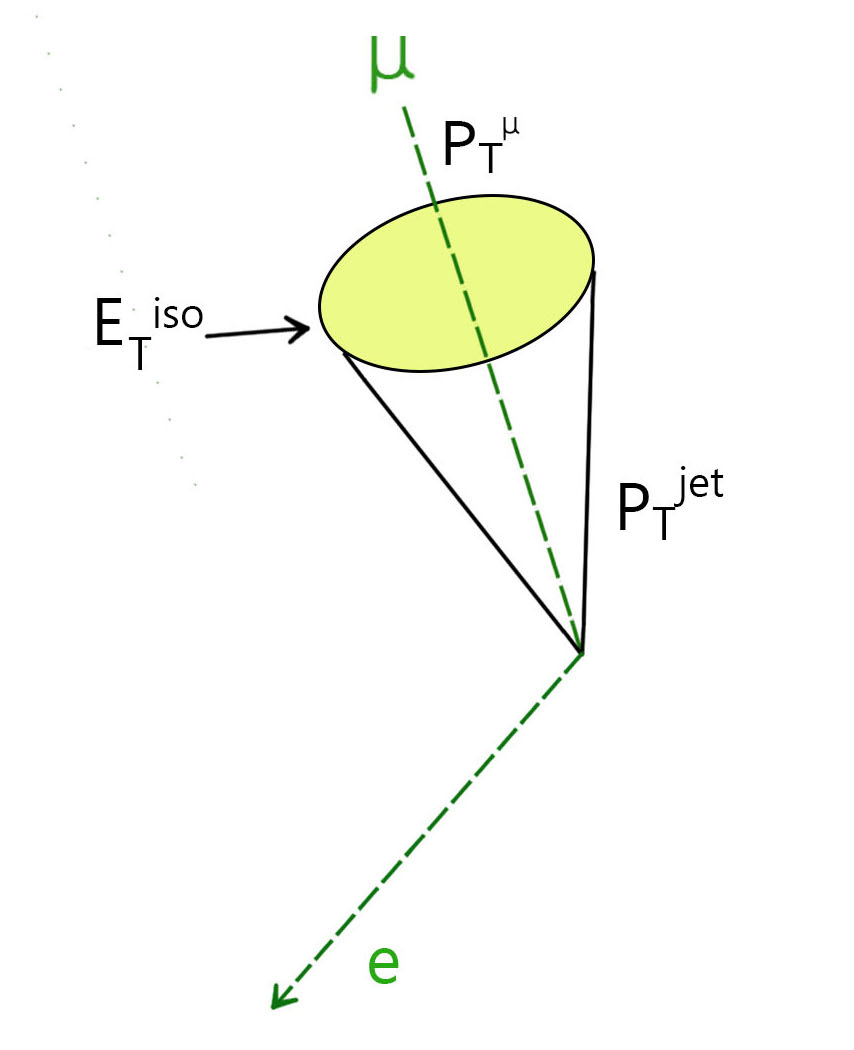
\includegraphics[scale=0.2]{images/iso_cone.jpg}
\caption{An illustration of an event where a prompt electron and a non-prompt muon, coming from a jet, fake a same-sign W-boson scattering event. Since the non-prompt muon is from a jet it is less likely to be isolated than than if it were prompt. Modified from \cite{ssWW_int_note}.}
\label{isolation_cone}
\end{figure}

\begin{figure}
\centering
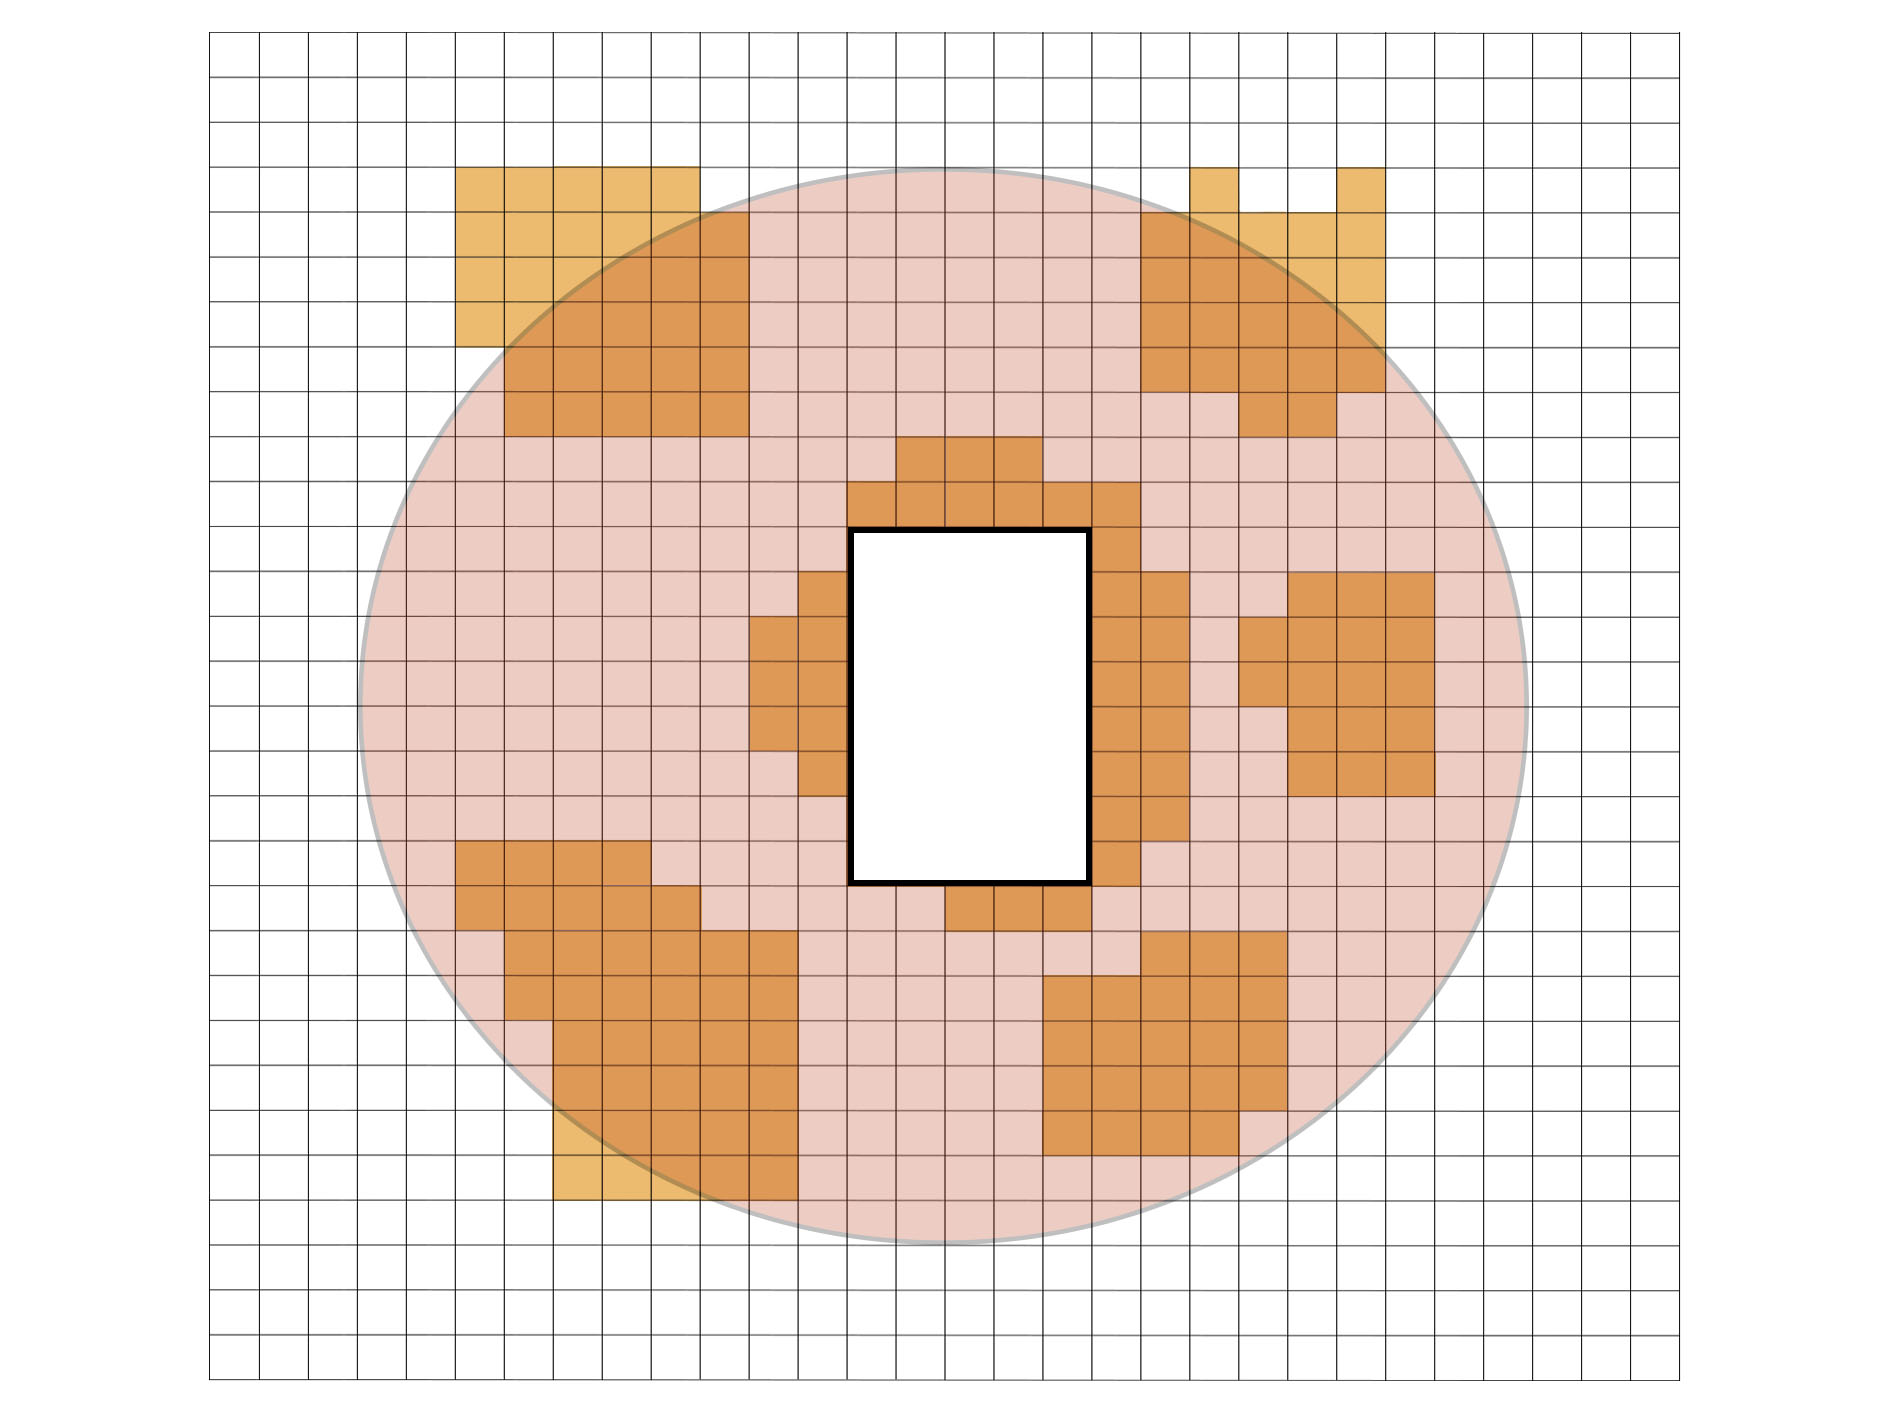
\includegraphics[scale=0.65]{images/topo_clusters.jpg}
\caption{An illustration of how the \textbf{topoetcone} variable is constructed. The grid in $\eta - \phi$ space represents the middle calorimeter cells. At the centre of the cone lies the incident lepton/photon. The topological clusters (coloured orange) are included in the calculation if their barycentre lies within the cone. The white $5 \times 7$ rectangle represents the cells subtracted in the calculation when using the \textbf{core57cells} technique. Modified from \cite{laplace}.}
\label{topo_clusters}
\end{figure}
\subsection{The ATLAS Isolation Selection Tool Working Points}
\label{AIST}
The isolation working points should be as independent of event topology as possible. Thus they are based on isolation variables using the smallest cone size $\Delta R = 0.2$, and for lepton track isolation \textbf{ptvarcone}. Motivated by this, the working points are based on the \textbf{topoetcone20} and \textbf{ptvarcone20} variables.
The official \emph{ATLAS Isolation Selection Tool} posses a number of official working points which can be used to accept or reject leptons with varying degrees of efficiency. The efficiency is defined, in the context of $Z \longrightarrow \ell \ell$ ($\ell = e/\mu$), as
$$\varepsilon =  \frac{N_{e/\mu}^{pass}}{N_{e/\mu}^{all}}, $$
where $N_{e/\mu}^{pass}$ is the number of electrons/muons originating from the hard process that pass the isolation requirement, while $N_{e/\mu}^{all}$ is the total number of electron/muons originating from the hard process. The process, $Z \longrightarrow \ell \ell$, is chosen due to its clean experimental signature.

These official working points can be classified as either:
\begin{itemize}
\item simple fixed cuts of the from $\mathbf{ptvarcone30} < X$ GeV,
\item so-called targeted efficiencies, with either gradient efficiency of 95$\%$ at $p_{T} = 20$ GeV and 99$\%$ at $p_{T} = 80$ GeV or flat efficiency of 99$\%$ in the $\eta-\phi$ plane. These lepton only working points are based on cut maps from $Z \longrightarrow \ell \ell$ Monte Carlo samples.
\end{itemize}
Many fixed cuts are applied to the fractional isolation (the isolation variable divided by $p_{T}$). These cuts are useful in that they are looser on high $p_{T}$ leptons and hence suited to searches for high $p_{T}$ objects. Only fixed isolation cuts are applied to photons.
Some example isolation working points are described in table \ref{iso_wps}.
\begin{table}
	\resizebox{\textwidth}{!}{\centering{\begin{tabular}{|c|c|c|c|c|}
	\hline
	Working Point & Objects & Calorimeter Isolation & Track Isolation & Combined Isolation \\ \hline \hline
	\textit{Loose} & all leptons & 99$\%$ & 99$\%$ & 99$\%$ \\ \hline
	\textit{Gradient} & leptons & $\varepsilon$=(0.1143$\times$$p_{T}$[GeV]+92.14)$\%$ & $\varepsilon$=(0.1143 $\times$$p_{T}$[GeV]+92.14)$\%$ & $\varepsilon$(25 GeV)=90$\%$, $\varepsilon$(60 GeV)=99$\%$ \\ \hline
	\textit{GradientLoose} & leptons & $\varepsilon$=(0.057$\times$$p_{T}$[GeV]+95.57)$\%$ & $\varepsilon$=(0.057$\times$ $p_{T}$[GeV]+95.57)$\%$ & $\varepsilon$(25 GeV)=95$\%$, $\varepsilon$(60 GeV)=99$\%$ \\ \hline
	\textit{FixedCutTightTrackOnly} & muons & - & cut:$\mathbf{ptvarcone30}/p_{T} < 0.06$ & - \\ \hline 
	\textit{FixedCutTightTrackOnly} & electrons & - & cut:$\mathbf{ptvarcone20}/p_{T} < 0.06$ & - \\ \hline
	\textit{FixedCutLoose} & electrons & cut:$\mathbf{topoetcone20}/p_{T} < 0.2$ & cut:$\mathbf{ptvarcone20}/p_{T} < 0.15$ & - \\ \hline
	\textit{FixedCutLoose} & muons & cut:$\mathbf{topoetcone30}/p_{T} < 0.3$ & cut:$\mathbf{ptvarcone30}/p_{T} < 0.15$ & - \\ \hline \hline
	\end{tabular}}}
\caption{Selected official working points for the ATLAS Isolation Selection Tool. \cite{isolation_working_points}}
\label{iso_wps}
\end{table}
The cone sizes for the isolation variables come in three sizes: $\Delta R = 0.2, 0.3, 0.4$ . Relevant isolation variables in this thesis are given a brief description below.
\begin{itemize}
\item \textbf{etcone}: calculated from the calorimeter cells in the given cone,
\item \textbf{topoetcone}: the sum of the $E_{T}$ of the topoclusters in the given cone,
\item \textbf{ptcone}: the sum of the $p_{T}$ of tracks in the given cone around the interested object; the tracks are required to have $p_{T} > 1$ GeV, $|z_{0} \sin \theta | < 3$ mm and pass the \textit{loose} track quality cut,
\item \textbf{ptvarcone}: has a maximum size, to stop it blowing up at low $p_{T}$; at larger values of $p_{T}$, \textbf{ptvarcone} has a smaller cone size than \textbf{ptcone}.
\end{itemize}